\section{Création du modèle de \glsfmtlong{mt}}
\label{sec.mt-model-creation}

La section précédente fournie une vue de la procédure de création d'un corpus parallèle pour la \gls{mt}.
Dans cette section, nous exploitons ce corpus pour créer et entraîner un modèle de \gls{nmt}.

\subsection{Création du modèle}
\label{subsec.mt-model-creation}

Comme discuté dans Section~\ref{sec.tech}, 
nous avons choisi d'utiliser PyTorch et \foreignlanguage{english}{PyTorch Lightning} pour la partie \gls{dl}.
La classe \verb|Transformer| qui représente notre modèle hérite donc de la classe
\verb|lightning.pytorch.LightningModule| qui elle-même hérite de la classe \verb|torch.nn.Module|.
L'Extrait de code~\ref{code.transformer-init} montre la méthode d'initialisation de cette classe.

\lstinputlisting[
    language=Python,
    caption={Méthode d'initialsation d'un transformeur.},
    label={code.transformer-init},
    firstline=12,
    firstnumber=1
]{assets/scripts/transformer-init.py}

La méthode \verb|__init__| prend en argument les hyperparamètres du modèle
(\verb|d_model|, \verb|nhead|, \verb|num_encoder_layers|, 
\verb|num_decoder_layers|, \verb|dim_feedforward| et \verb|dropout|)
ainsi que des paramètres de configuration de l'entraînement et de l'inférence
(\verb|source_vocab_size|, \verb|target_vocab_size|, \verb|source_pad_idx|, \verb|max_len| et \verb|lr|).

L'appelle à la méthode \verb|super().__init__()| a l'effet de construire par défaut un \verb|LightningModule|.
Les lignes qui suivent cette instruction permettent d'initialiser ce module 
en définissant les couches qui le composent.
Parmi ces couches, la plus importante et \verb|self.transformer|,
un objet de la classe \verb|nn.Transformer|.
Tous les autres modules sont des couches de prétraitement (encodage positionnel)
ou de post-traitement (projection linéaire).
La Figure~\ref{fig.arch} montre le graphe de calcul du modèle résultant.

\begin{table}[hbt]
    \begin{center}
        \begin{tabular}{|l|l|l|l|}
            \cline{2-4}
            \multicolumn{1}{c|}{}& \verb|Name|& \verb|Type|         & \verb|Params|                     \\
            \hline
            0                    & \verb|input_embedding|           & \verb|Embedding|          & 320 K \\
            \hline
            1                    & \verb|input_position_embedding|  & \verb|Embedding|          & 6.4 K \\
            \hline
            2                    & \verb|output_embedding|          & \verb|Embedding|          & 320 K \\
            \hline
            3                    & \verb|output_position_embedding| & \verb|Embedding|          & 6.4 K \\
            \hline
            4                    & \verb|transformer|               & \verb|Transformer|        & 201 K \\
            \hline
            5                    & \verb|transformer.encoder|       & \verb|TransformerEncoder| & 75.8 K\\
            \hline
            6                    & \verb|transformer.decoder|       & \verb|TransformerDecoder| & 126 K \\
            \hline
            7                    & \verb|linear|                    & \verb|Linear|             & 325 K \\
            \hline
            8                    & \verb|dropout|                   & \verb|Dropout|            & 0     \\
            \hline
        \end{tabular}
        \ \\[.5cm]
        \begin{tabular}{ll}
            1.2 M & Paramètres entraînables       \\
            0     & Paramètres non entraînables   \\
            1.2 M & Paramètres totaux             \\
            4.719 & Taille totale estimée (en Mo) \\
        \end{tabular}
    \end{center}
    \caption{Résumé du modèle.}
    \label{tab.model-summary}
\end{table}

En utilisant les valeurs proposées dans le Chapitre~\ref{chap.conception} pour les hyperparamètres :
\[
    \begin{array}{l}
        d_{\mathrm{model}} = d_{\mathrm{FFN}} = 64\\ 
        N_{\mathrm{head}} = 4\\ 
        N_{\mathrm{encoder}} = N_{\mathrm{decoder}} = 3
    \end{array}
\]
nous obtenons un modèle dont la Table~\ref{tab.model-summary} résume les paramètres par couche.

\begin{figure}[htb]
    \begin{center}
        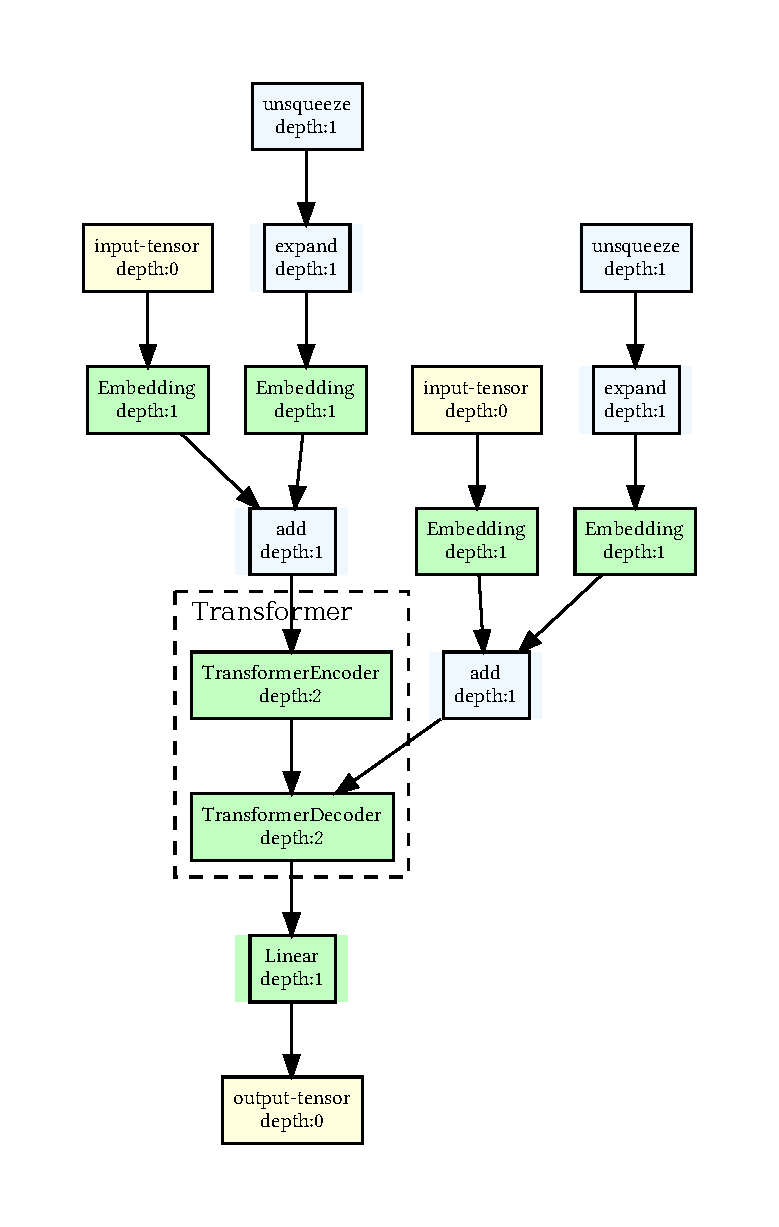
\includegraphics[width=.6\textwidth]{assets/pdf/arch.pdf}
    \end{center}
    \cprotect\caption[Graphe de calcul du modèle définit dans la classe \verb|Transformer|]%
    {Graphe de calcul du modèle définit dans la classe \verb|Transformer| \((\text{profondeur} = 2).\)}
    \label{fig.arch}
\end{figure}